\documentclass{article}
\usepackage[utf8]{inputenc}
\usepackage[margin=1in]{geometry}
\usepackage{mathtools,setspace,indentfirst,graphicx,float,hyperref,courier,color}
\usepackage{fancyhdr} % for header
\usepackage{listings}
\usepackage[english]{babel}
\usepackage[backend=biber,style=numeric]{biblatex}
\addbibresource{sources.bib}

\doublespacing{}

\fancyhf{}
\pagestyle{fancy}

\lhead{N Batista, M Inciong, F Truncale}
\chead{\thepage}
\rhead{Fall 2017}
\renewcommand{\headrulewidth}{0pt} % remove the horizontal line along the header

\lstset{%
  basicstyle=\ttfamily,
  captionpos=b,
  frame=tb,
  tabsize=2,
  showstringspaces=false,
  commentstyle=\color[RGB]{24,135,64},
  keywordstyle=\color{blue},
  stringstyle=\color{red}
}

\begin{document}

\thispagestyle{empty}

\begin{titlepage}
  \vspace*{\fill} % i copied this off stackexchange so no i don't know what that asterisk does.
  \begin{center}
    {\Huge Final Report --- Optimization of Subgraph Isomorphism Algorithm}\\[0.4cm]
    {\huge by Nelson Batista, Max Inciong, Francesca Truncale}\\[0.5cm]
    {\huge Senior Project II}\\[0.4cm]
    {\huge Professor Jianting Zhang}\\[0.4cm]
    {\LARGE Fall 2017}
  \end{center}
  \vspace*{\fill}
\end{titlepage}

\pagenumbering{roman}
%table of contents
\tableofcontents

\newpage

\pagenumbering{arabic}
\setcounter{page}{1}

%\addcontentsline{toc}{section}{Introduction}
\section{Introduction}

The goal of this project is to understand and optimize an algorithm for solving the NP-complete problem of subgraph isomorphism.

  \subsection{Background}

  An \textit{isomorphism} between two graphs is a mapping from the vertices of one graph, say $G$, to another graph, say $H$, such that any two vertices which are adjacent in $G$ are mapped to vertices which are adjacent in $H$. The subgraph isomorphism problem, in turn, is the problem of determining whether an isomorphism exists between a graph $G$ and any of the subgraphs of a larger search graph, $H$. The issue that makes the subgraph isomorphism problem so difficult to solve for a particular pair of graphs is cycling through the main graph and expanding each node within the graph and checking if each of the generated subgraphs formed from each node is isomorphic to the control graph.

  Fortunately, many attempts exist to solve the subgraph isomorphism problem. Among the earliest of these is the famous \textit{Ullmann Algorithm}, proposed by Julian R. Ullmann in his 1976 paper, \textit{An Algorithm for Subgraph Isomorphism}. He first describes a basic, naive approach to finding a mapping from the vertices of a graph to a subgraph of a larger graph. He goes on to define a ``refine'' procedure to dramatically reduce the number of possible mappings that must be checked.\cite{ullmann} These will be covered in greater detail in the next section.

  The goal of our project was to take this algorithm and improve its performance. Subgraph isomorphism is an expensive problem to solve, and finding multiple possible isomorphisms from one graph to subgraphs of another is even more expensive, so even slight improvements in the algorithm's performance is likely to lead to large performance improvements in any large-scale program which needs to use it often.

  \subsection{Motivation}

  Our reasoning for choosing this topic for our project is an apparent lack of especially efficient algorithms for solving the subgraph isomorphism problem. Solutions to the subgraph isomorphism problem are often used to detect similarities in chemical compounds,\cite{ullmann} which may shed light on some of their properties. If this process needs to be done, for example, on a very large database of chemical compounds, or less frequently for several very large compounds, the process may take a very long time to complete. It would be very beneficial to improve the performance of this algorithm, even if only slightly, so that these sorts of use cases can still be handled in a more reasonable amount of time.

  \subsection{Data Set}

  The primary graph used to test the algorithm and its performance is an undirected graph consisting of ``friends lists'' from the social media website, Facebook. Each node of the graph represents a unique user, and, if two nodes are adjacent, then their corresponding users are friends on Facebook.\cite{fbgraph}

  The graph contains 4,039 nodes and 88,234 edges. The relatively large size of the graph makes it well-suited to use for collection of performance data. As we shall see, the Ullmann algorithm takes a rather long time to complete with a graph of this size, allowing any optimizations and/or parallelizations to be readily apparent.

\section{Ullmann Algorithm}

  \subsection{Naive Approach}

  The paper begins, as many do, with a definition of terms that will be used throughout. We have repeated them here for the sake of clarity later on. We begin by noting that the algorithm models the search for a possible mapping by having all possible mappings as nodes on a tree, on which a depth-first search is performed to find a solution.

  The subgraph isomorphism problem is defined as the problem of finding all isomorphisms between a graph $G_\alpha = (V_\alpha, E_\alpha)$ and subgraphs of another graph $G_\beta = (V_\beta, E_\beta)$, with $(V_\alpha, E_\alpha)$ and $(V_\beta, E_\beta)$ being the set of vertices and edges of $G_\alpha$ and $G_\beta$, respectively. The number of vertices and edges of $G_\alpha$ and $G_\beta$, respectively, are $(p_\alpha, q_\alpha)$ and $(p_\beta, q_\beta)$.

  The \textit{adjacency matrix} for graph $G_\alpha$, $[a_{ij}]$, is defined by:

  \[ a_{ij} = \begin{cases}
                1 & \textrm{ if } i \neq j \textrm{ and } i,j \textrm{ share an edge} \\
                0 & \textrm{ otherwise}
  \end{cases}
  \]

  The adjacency matrix for graph $G_\beta$, $[b_{ij}]$, is defined equivalently.

  Notably, we have the $p_\alpha \times p_\beta$ matrix $M$, which is a binary matrix of assignments (mappings) from $V_\alpha$ to $V_\beta$. That is, if $m_{ij}$ is 1, then vertex $i$ in graph $G_\alpha$ could possibly be mapped to vertex $j$ in $G_\beta$. Otherwise $m_{ij}$ is 0. M has a few interesting properties as a result, which will soon be apparent.

  Finally, we come to $d$, which is simply algorithm's current depth in the search tree. The algorithm starts at $d = 0$, and terminates when $d = p_\alpha$. The matrix $M$ at a particular depth $d$ is denoted as $M_d$, with solutions to the working instance of the subgraph isomorphism problem being the set of assignments from $V_\alpha$ to $V_\beta$, contained within matrices $M_{p_\alpha}$. $M_0$ is generated by the following formula:

  \[ m_{ij} = \begin{cases}
    1 & \textrm{ if degree} (j \in G_\beta) \geq \textrm{ degree} (i \in G_\alpha) \\
                0 & \textrm{ otherwise}
  \end{cases}
  \]

  Each step of the computation consists of setting all but one of the values of one of the rows of $M$ to 0, and then checking whether exactly one 1 exists in each row. If it does, we have found an isomorphism, since each vertex of $G_\alpha$ has been mapped to exactly one vertex of $G_\beta$. If it does not, then we continue onto another row of $M$ and check again. If we have reached the point where we cannot perform the operation on a row of $M$ without violating the condition that each \textit{column} of $M$ contains at most a single 1 (a vertex of $G_\beta$ cannot be mapped from multiple vertices of $G_\alpha$), then we backtrack to a previous version of $M$ and try to change the column that we set to 1 in the current row. After exhausting all columns, we conclude there cannot be an isomorphism, since at least one vertex of $G_\alpha$ cannot be mapped to any vertex of $G_\beta$.\cite{ullmann}

  \subsection{``Refine M'' Procedure}

  In the most basic algorithm, the entire tree is searched, including branches which cannot possibly contain a solution at any depth. This is a large number of $M$ matrices to evaluate, so Ullmann introduces a ``refine M'' procedure to reduce the number that must be checked by eliminating nodes of the tree which cannot contain a solution.

  The procedure is actually quite simple. We iterate through each 1 $m_{ij}$ in $M$ and check whether, for each neighbor of the vertex in $G_\alpha$ corresponding to $i$, there exists at least one possible assignment from it to a neighbor of the vertex in $G_\beta$ corresponding to $j$. If this condition does not hold, the 1 is changed to a 0. Since doing so may render other 1s invalid, we repeat the refine procedure on the modified $M$ until running the procedure does not change it any further, indicating that the refinements do not produce any new invalid 1s. This obviously involves several layers of nested loops, adding considerable overhead to the overall algorithm. However, this overhead is very little considering the number of possibilities that are subsequently eliminated, making it a very worthwhile operation to perform regardless.

  This refine M procedure is run both on the initial $M$ as well as each of $M_d$, greatly reducing how many iterations we must perform to see that a particular mapping is invalid.

\section{Alternative Algorithms}

  \subsection{VF2 Algorithm}

  % this whole section looks like you copied it verbatim out of notes you took while skimming a paper
  % i'd confuse it for a chat log if not for the fact that there's actual capitalization
  One algorithm that we considered using was the VF2 Algorithm, which was developed by Cordella, Foggia, Sansone, and Vento.

  Given two graphs $G_1(n_1,b_1)$ and $G_2(n_2,b_2)$ and Mapping $M : n_1 \times n_2$, a subset mapping solution $M(s)$ takes two subgraphs $G_1(s)$ and $G_2(s)$, obtained by selecting from $G_1$ and $G_2$
  only the nodes included in the components of $M(s)$, and the branches connecting them.
  % this sentence jesus christ
  The following algorithm is defined by the paper to implement VF2.

  \begin{figure}[H]
    \centering
    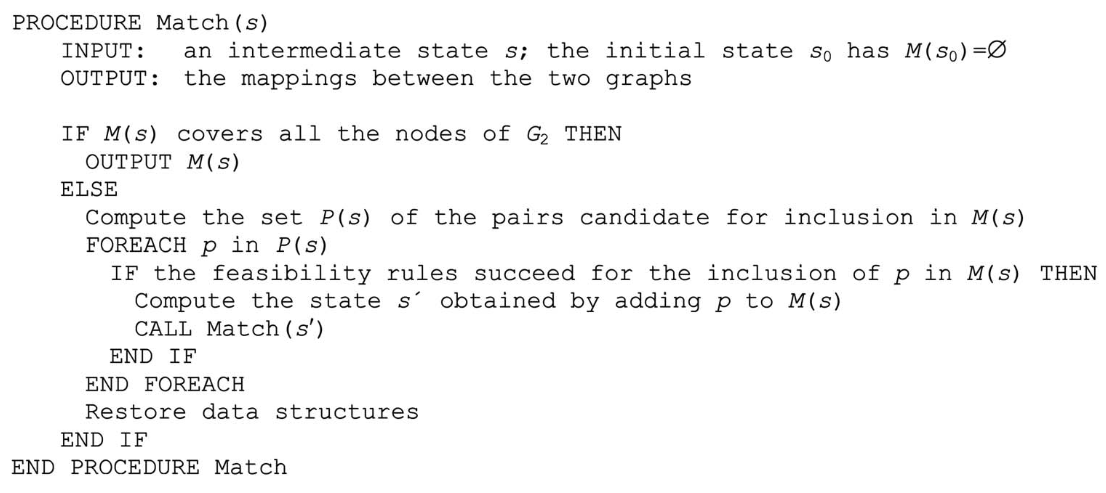
\includegraphics[scale=0.7]{images/vf2_rules.png}
    \caption{Description of the VF2 Algorithm.}
    % use \ref{fig:vf2algo} to refer to this figure in text
    % not that you do anyway
    \label{fig:vf2algo}
  \end{figure}

  For each mapping $(m,n)$, VF2 applies five feasibility rules to the current state and the pair to be added. These rules are denoted as: $R_{pred}, R_{succ}, R_{in}, R_{out},$ and $R_{new}$.

  Only if all feasibility rules are satisfied is $(n,m)$ added to the set of mappings $M(s)$.

  The general form of the feasibility function is defined as:

  $F_{syn}(s,n,m) = R_{pred} \land R_{succ} \land R_{in} \land R_{out} \land R_{new}$

  $R_{pred}$ and $R_{succ}$ represent the predecessors and successors respectively of a given node \texttt{n}  in a graph.

  The other three feasibilty rules are meant to prune the tree
  $R_{in}$ and $R_{out}$ are both 1 step ahead look ahead while $R_{new}$ is a 2 step look ahead.

  "Look ahead" refers to the \texttt{k-look-ahead} rules defined in the paper. They are used to reduce the number of states generated, by checking in advance if a consistent state \texttt{s} has no consistent successors after \texttt{k} steps.

  The feasibility rules are defined as the following:

  \begin{figure}[H]
    \centering
    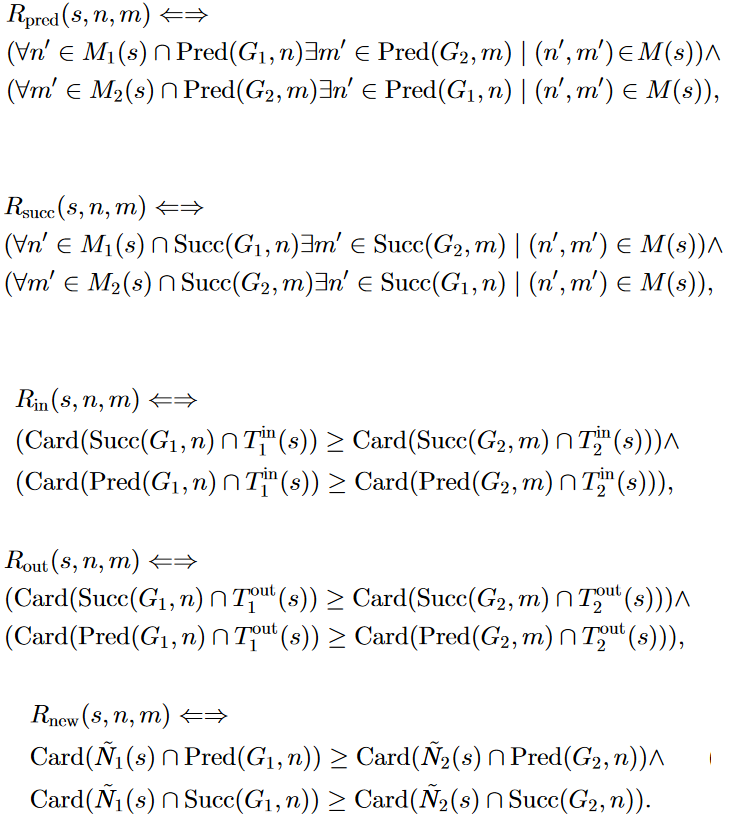
\includegraphics{images/vf2_algo.png}
    \caption{Description of the creation of feasbility rules.}
    \label{fuckyou}
  \end{figure}

  In comparison to the Ullman algorithm, it appears that when working with greater than 200 nodes, VF2 becomes more efficient than the it.

  The time complexity of VF2 is $O(n^2)$ at best, $O(n!n)$ at worst.
  Ullman's algorithm ranges from $O(n^3)$ to $O(n!n^2)$.
  % this was broken btw
  % when you have a list of authors you're supposed to use and (the literal word "and") to separate them in the bib entry
  % that's how biber recognizes different authors
  % the way you had it made the entries invalid so the citations wouldn't show up
  \cite{cordella}

  \subsection{RI Algorithm}

  For this algorithm, we need to generate all possible maps between two graphs, then check if any of those maps is a subgraph isomorphism.

  The maps can be represented using a \textit{search space tree}, which has a dummy root. Each node represents a possible match between a vertex in graph $G$ (which is referred to as the pattern graph) in the target graph $G'$.

  Unlike other algorithms, RI orders the vertices of the pattern graph in a way that maximizes the chance that a partial path will be removed. The idea is to introduce edge constraints as early as possible, and are modeled only on the pattern graph.

  RI is also modeled for directed graphs, which allows for more pruning since $(u,v)$ does not imply $(v, u)$ (where $u, v$ are vertices).

  The majority of the work is performed in a greedy algorithm called \texttt{GreatestConstraintFirst}, which is used to find a good sequence of vertices based on the number of neighbors a vertex has.

  Using the results of \texttt{GreatestConstraintFirst}, the following isomorphism rules remove unfeasible paths:

  \begin{figure}[H]
    \centering
    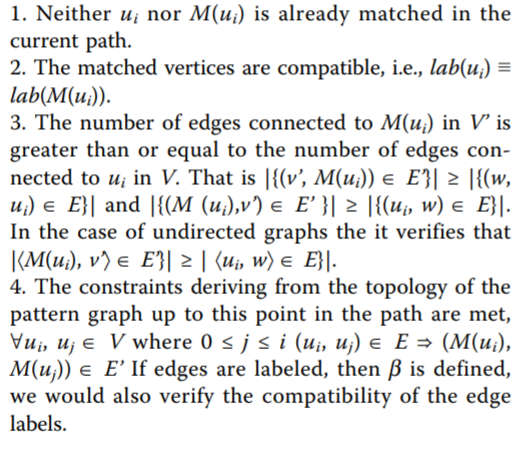
\includegraphics{images/ri_rules.png}
    \caption{RI Feasibility Rules}
    \label{ri_feas}
  \end{figure}


  The algorithm does not have a dedicated pruning function, which is another factor for the increase in performance when compared against other algorithms (such as VF2); instead, pruning is done through the matching process.\cite{bonnici}

\section{Implementation of the Algorithm}

The full source code for all versions can be found in the appendix.

  \subsection{Python Implementation}
  The Python code is based largely on an implementation of the Ullmann algorithm provided by an answer on the website \textit{StackOverflow}.\cite{pyiso} It would not run in its original form, so a few adjustments were needed.

  \begin{lstlisting}[language=Python,caption={Function used to determine whether an isomorphism exists.}]
  def find_isomorphism(graph, subgraph):

      assignments = []
      possible_assignments = [[True]*graph.n_vertices() \
                    for i in range(subgraph.n_vertices())]
      if search(graph, subgraph, assignments, possible_assignments):
          return True
      return matches
  \end{lstlisting}

  The main function is \texttt{find\_isomorphism}, which is depicted above. It calls the function \texttt{search}, which performs the actual work of finding an isomorphism.

  The \texttt{search} function runs  the \texttt{update\_possible\_assignments} function. This particular function has been the subject of refining over the course of the project. At the time of the python implementation, it was the most significant bottleneck.

  This was mostly due to the usage of the \texttt{has\_edge} method of the graph class, shown below.

  \begin{lstlisting}[language=Python,caption={Code for the \texttt{has\_edge} method of our graph class.}]
  def has_edge(self, vert1, vert2):
       """ Checks if edge connecting vert1 and vert2 is in the graph
       """
       #if adjacent, there's an edge
       return ({vert1, vert2} in self.adjacencies)

  \end{lstlisting}

  This method calls the built-in \texttt{in} function of Python lists, which has a runtime complexity of O(n).\cite{bigopy} Thus, the \texttt{has\_edge} method of the Python implementation is O(n).

  \subsection{Initial C++ Implementation}

  The initial C++ implementation was based entirely on the Python implementation. Indeed, it represented our best attempt to ``translate'' the Python code to C++. As one might imagine, it was riddled with compilation errors. That said, we did manage to get it to run, and analysis indicated it performed little better than the Python equivalent. We suspected this was because it retained the same issue that the Python implementation had: calling \texttt{has\_edge}, an O(n) method, countless times. This motivated a significant improvement.

  \subsection{Improved C++ Implementation}

  The improved C++ implementation represents a significant milestone in our project, as it not only improved upon the clarity of the isomorphism algorithm, but also resulted in a much cleaner graph class, with edges implemented as an adjacency matrix. This makes the \texttt{has\_edge} function O(1), as it consists of simply looking up whether the given vertices share an edge by checking the matrix. This makes its repeated use in \texttt{refine\_possible\_assignments} much more acceptable, a fact which is reflected in the performance.

  We also have stored vertices in such a way that each vertex is also stored along with its degree, allowing quick and easy lookup of a vertex's degree.

  The improved C++ implementation follows a bit of a loose interpretation of Ullmann's description of the algorithm. A version which used the \texttt{goto} command with labels was considered, to more closely match said description, but was scrapped in favor of a more conventional approach

  \subsection{Options for Parallelization}

    % todo needs to be cleaned up
    % lots of sloppy/awkward phrasing
    % some parts unclear
    % lots of missed opportunities to go into detail
    \subsubsection{GPGPU}
    % talk about gpgpu in general
    When GPUs (graphics processing units) began including programmable shaders and support for floating point arithmetic, they became capable of doing calculations on matrices or vectors. While early GPGPU programming (General Purpose computing on Graphics Processing Units) required formulating problems as graphics primitives, there are now APIs to avoid the translation.

    One of these APIs is CUDA, which is a proprietary parallel computing platform created by Nvidia. Source code written in CUDA uses C++ syntax, and only Nvidia GPUs are enabled for CUDA. It has the potential to use more than the available cores from a standard CPU, and is only limited by the number of CUDA cores that a GPU contains. This ranges from 8 to 5760 (at the time of writing, the Titan Z has 5760 CUDA cores). The main difference between using CUDA and OpenMP is that CUDA has access to more threads. OpenMP relies on using the cores of a CPU to do parallel work; as a result, work is sped up by approximately a factor of $2^8$, depending on how many cores a computer has.

    A similar API is OpenCL (Open Computing Language), a framework that allows programs to execute accross multiple types of processing hardware. Similar to CUDA, source code is written using C-like syntax. Unlike CUDA, it does not require specialized hardware; OpenCL is an open standard, which can be used across AMD, Nvidia, and Intel GPUs, as well as other processors.

    \subsubsection{MPI}
    % the function runs once on each machine.
    % and the machines have to communicate with each other to combine their results
    % further reducing the potential speedup
    % talk about that for a bit
    MPI stands for Message Passing Interface. This utilizes multiple machines in order to parallelize the work. Unfortunately there is a huge difference between parallelization using threading and MPI. With MPI, the function runs once on each machine. This means that in order to increase effectiveness, the workload must be balanced among the machines, otherwise some machines might do much more work than other machines, reducing the effective time saved, as a program running in parallel is only as fast as its slowest processor. One cannot simply throw MPI onto a program and expect it to go faster by some factor. In the case of graph and subgraph isomorphism, we would have to split the work based on which sections of the graph take longer.

   % "system of machines"
   % last sentence is a little wonky
    Theoretically it is possible to combine MPI with OpenMP in order to increase the efficiency. However, our team did not have a network of machines in order to fully utilize MPI. If we did, the time it would take to find an isomorphism would decrease by at most a factor based on the number of processors used, multiplied by the number of cores in each processor capable of using OpenMP.

    \subsubsection{SIMD}
    % he's trying to explain vector instructions here
    SIMD stands for single instruction multiple data. This system uses a series of data types found in specific systems. Examples of SIMD include AVX, SSE, and ARM-NEON vector instructions. These instructions allow for a certain datatype that could hold multiple values and perform operations on multiple pieces of data at once. These operations can either be between two vectors or between values within the vectors. We would have to drastically alter the data structures we currently have in place to incorporate SIMD datatypes.

    % include openmp here to justify why we went with it over the others
    \subsubsection{OpenMP}

  \subsection{Optimizations through OpenMP}
  OpenMP utilizes the multiple cores of a computer's processor in order implement multithreading to run related tasks in parallel. We intend to use it where the bottlenecks in our algorithm are to improve the algorithm's performance. The default number of cores for many computers is four. We intend to place the parallelisms where there tend to be a large number iterations, specifically in loops. This means that, theoretically, the program should run four times faster than without multithreading, using our earlier assumption of four processor cores allotted to the algorithm. It is more likely that it will be approximately 3 to 3.5 times faster, since we may not be able to completely parallelize the bottlenecks as intended. Additionally, using OpenMP, as is the case with any parallelization method, comes with a certain amount of overhead in separating the work to be done. There is also the issue of load balancing: making sure that each thread is performing approximately the same amount of computation so that no thread is idling.

  The most important place to place the OpenMP is in the \texttt{refine\_possible\_assignments} function. This function is where the majority of the algorithm's computation takes place, as it has several layers of nested loops, each iterating through vectors which may be very large, depending on the sizes of the graphs being examined. Ideally, we want to balance the loads such that each processor core does an equal amount of work, so as to maximize the amount of parallelization done. However, while we may simply parallelize every iterative process, that might not be efficient enough. Ideally, we would further parallelize in nodes of the search tree which have many possible assignments.

  \subsection{Sample Run}

  For visualization purposes, we have provided a sample run of the algorithm. For simplicity, only the C++ implementation is seen here. The graphs used are very simple, as this is only for demonstration. The following is the list of edges defining the search graph:

  \lstinputlisting[caption={Search graph used for walkthrough.}]{../../src/toy1.edges}

  And the following is the subgraph we will be searching for an instance of in that graph:

  \lstinputlisting[caption={Subgraph being searched for in search graph.}]{../../src/toy1sub.edges}
  % TODO this
\section{Performance}

For all of our measurements, we used the worst-case input: the Facebook graph mentioned previously as the search graph, and that same graph (or, equivalently, any isomorphic graph of the same size) as the ``subgraph.'' This would take the longest of the graphs available to us, since it requires the algorithm to assign the greatest number of vertices (all of them) before returning, and, since the graphs are indeed isomorphic, there is no chance of \texttt{refine\_possible\_assignments} returning false, which would allow us to skip a large amount of work.

  \subsection{Python Implementation}
  The Python implementation was very inefficient, but it was necessary for us to understand what we had to do for a C++ implementation. It took between 13 and 16 seconds to determine if an isomorphism existed.

  We used the Python \texttt{cProfile} library to measure the performance of our Python implementation. The documentation is available at \url{https://docs.python.org/3.5/library/profile.html}. A typical run of the \texttt{find\_isomorphism} function timed by \texttt{cProfile} produces the following output:

  \begin{figure}[H]
    \centering
    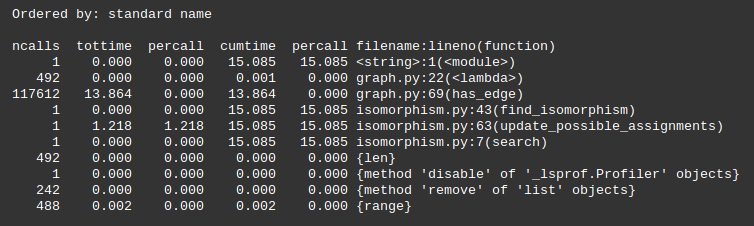
\includegraphics[scale=0.6]{images/perf}
    \caption{Sample run of the Python implementation of subgraph isomorphism.}
  \end{figure}

  \subsection{C++ Implementation}
  The source code used to test the performance of the C++ implementations can be found in the appendix. We used Linux's \texttt{perf\_event\_open} system call, which allows for high-precision performance monitoring. The only part of the program which is timed is the call to \texttt{find\_isomorphism}.

  The C++ implementation, due to the improvement of \texttt{has\_edge}'s runtime, runs significantly more quickly than the Python implementation; it runs in about 8 seconds, compared to about 16 seconds for the Python implementation. This is about twice as fast, even without any parallelisms. However, we found it was generally more precise to measure the number of CPU clock cycles taken for the algorithm to complete, so we measured that instead. The output of the program used to measure this is below:

  \subsection{OpenMP Optimization}
  The OpenMP code performs very well compared to the non-parallelized version.

\section{Conclusion}
  Over the coming two weeks, we should have completed the OpenMP parallelizations and thoroughly tested the performance of the resulting program. We will also be much more in-depth in the explanation of the Ullmann algorithm. We also hope to use a more precise method of getting performance information for the C++ implementation, as our current method is rather volatile.

\section{Appendix}
  \subsection{Python Code}
    \subsubsection{Graph Class}
      \lstinputlisting[language=Python,caption={Python graph class.}]{../../src/pythonvers/graph.py}
    \subsubsection{Subgraph Isomorphism Algorithm}
      \lstinputlisting[language=Python,caption={Python algorithm to find isomorphism.}]{../../src/pythonvers/isomorphism.py}
    \subsubsection{Main}
      \lstinputlisting[language=Python,caption={Python main function to process arguments and run the ismorphism algorithm.}]{../../src/pythonvers/main.py}

  \subsection{C++ Code}
    \subsubsection{Graph Class}
      \lstinputlisting[language=C++,caption={C++ graph class.}]{../../src/cvers/graph.cpp}
    \subsubsection{Subgraph Isomorphism Algorithm}
      \lstinputlisting[language=C++,caption={C++ algorithm to find isomorphism.}]{../../src/cvers/isomorphism.cpp}
    \subsubsection{Main}
      \lstinputlisting[language=C++,caption={C++ main function to process arguments and run the ismorphism algorithm.}]{../../src/cvers/main.cpp}

  \subsection{OpenMP Code}
    \textbf{Note:} Since the OpenMP version of our algorithm uses the same graph class and \texttt{main.cpp}, we have omitted them from this section.

    \subsubsection{Subgraph Isomorphism Algorithm}
      \lstinputlisting[language=C++,caption={C++ algorithm to find isomorphism, with parallelisms through OpenMP.}]{../../src/openmp/isomorphism.cpp}

  \subsection{Code Used to Check Performance of C++ code}
    % if you've got a better caption be my guest
    \lstinputlisting[language=C++,caption={Code used to check performance of C++ code}]{../../src/cvers/perf.cpp}

  \printbibliography[heading=bibintoc,
                     title={References}]

\end{document}
